\chapter{Related Works}

\section{Electroencephalogram}
Elektroensefalografi(EEG) is a test that is widely used to detect brain waves. This signal is recorded by the deviceElectroencephalography, Is hardware that functions record the electrical activity of a brainwave. The working principle of this EEG detects activity electricity from the brains of people with that recorded by silver electrodes that are installed by trained technicians in the scalp. In this study, participants brain activity was observed using an electroencephalogram (EEG) while each of the participants completed spatial ability assessments\cite{ruesch2017understanding}
\par
The medical community using EEG, among others for the diagnosis of diseases associated with the brain and psychiatric disorders. EEG is also applied to detect patterns of mind or mental condition of a person. Visual observation of the EEG signal directly is challenging given the EEG signal amplitude is low and thus a very intricate pattern. Besides, the EEG signals are strongly influenced by a variety of variables, such as mental state, health, the activity of the patient, the recording environment, electrical interference from other organs such external stimuli, and the age of the patient. The nature of EEG signals is generally non-stationary and random, so that adds to the complexity in the processing of EEG signals. However,\cite{perry2017effects}

\section{Brain}
The brain is a central nervous system consisting of billions of cells called neurons. Each neuron communicates with each other and emits electric waves or commonly known as brain waves. Brain waves can be measured using an electroencephalogram (EEG). Brain waves produce frequencies that vary between 0.5-30 Hz and are classified into delta, theta, alpha, and beta waves. Each stream has different characteristics and shows a person's mental state. where every brain activity is very dependent on the situation of drug users, and where loyal users must be the brain waves produced vary between brain waves produced by the drug user, and where the state of the brain mostly produces internal rhythms from outside the user's drug awareness.\cite{mccormick2015brain}

\subsection{Brain Waves}
Brain waves can be measured with equipment Electroencephalograph (EEG). It is known that the frequency of brain waves generated by neurons varies between 0-30 Hz and is classified into a delta wave, theta, alpha, and beta. Each stream has different characteristics and indicate a person's mental condition. Human brain waves have different frequency and amplitude range – different\cite{liu2015plasticity}, so it is divided into several types of waves as follows:

\begin{enumerate}
    \item Delta waves
    \par
   Delta waves have frequency waves that are worth 1.5 <4 Hz. Delta waves are one of the slowest waves of other brain waves, in this condition a person's body carries out a process of self-healing, repairing damage to body tissues, and actively producing new cells when a person is sound asleep\cite{assenza2015wakefulness}
   
    \item Theta waves
    \par
    Theta waveform has a frequency value between 4 -8 Hz with a voltage amplitude reaches 10 μV. These waves are generated when a person is experiencing light sleep or drowsiness\cite{chiu2015complexity}
    
    \item Alpha waves
    \par
   Alpha waves have a frequency value between 8-13 Hz, where this frequency is a control of the body or conscious and subconscious mind where a person can remember a dream or more significantly someone does meditation (mild meditation)\cite{okumura2006amplitude}
   
    \item Beta waves
    \par
   Types Beta waves have a frequency of between 14-19 Hz and 20-30 Hz in beta waves indicating that a person is experiencing mental wakefulness or someone can control himself or think that he is tired because a lot of work presses or complicated problem solving\cite{malik2018brain}
   
    \item Gamma waves
    \par
    Gamma waveforms have a frequency value of 30-40 Hz. These waves are produced when someone experiences extraordinary mental activity or can be said to be bad usually someone who is undergoing a match, is panicking or is scared\cite{martini2018spatial}
    
    \begin{figure}[h!]
\centering
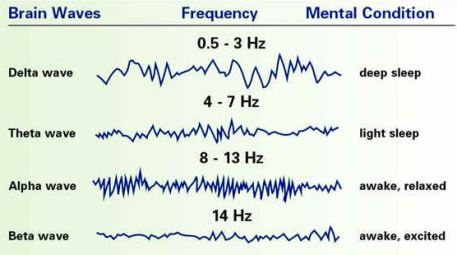
\includegraphics[scale=0.6]{figures/mengetahuigelombangotak.jpg}
\caption{Form biolistic Brain Signals}
\label{labelgambar1}
\end{figure}
\end{enumerate}

\section{MATLAB}
MATLAB is a high-level programming language for applications in various fields, such as numeric computation, analysis, and data visualization software and algorithm development, and design of the model system. (MathWorks, 2017) MATLAB toolbox is complemented by a wide range to support specific tasks, either developed directly by MathWorks and third parties. In this study, the toolkit is used field trip.

\par
A field trip is an open source software for EEG analysis, magnetoencephalography (MEG), electrophysiological data and more. The software supports a variety of functions for the study of EEG as a pre-processing of data, ERP analysis, classification, and others. Here is a preview of the software is MATLAB icon 2017 in Figure 2.2

\section{Feature Extraction}
\par
Is a feature extraction stage signal processing into a vector that contains the relevant values, so that the message can be analyzed and taken the information for further processing? In this phase, the raw signal data will be filtered by a bandpass filter, so that the signal will be passed the signal value of the frequency based on the sampling frequency is 5-30 Hz. Signal filter results are still in the time domain so that the information can not be retrieved. Furthermore, the signal is converted to the frequency domain peril by using the P-300. These values are ideally able to provide the information contained in the EEG signals associated mental states to be identified and reject artifacts and other benefits that are not relevant (Lotte, 2014). Examples of the signal features include statistical feature frequency (Abootalebi et al.,(Subasi, 2014; Panel al, 2014, Ramirez-Cortes et al., 2010).
\par
In the process of classification features, the features have been extracted signals are categorized by class or label set. These classes are related to mental states to be identified (Fraser, 2014). EEG signal processing is generally done automatically, not least in the process of classification features and optimizes the system. Menuurut Lotte (2014), there are two processes in the design of the EEG signal classification system based machines, namely:

\begin{enumerate}
    \item raining is the stage of system optimization through parameter tuning features and training system.
    \item Testing a testing stage classification system has been trained * with using data that is not previously known.
\end{enumerate}

